\documentclass[book.tex]{subfiles}
\begin{document}
\section{Source Code}
The game engine source code was released on July 21st, 1995. Twenty years later it is still there on id software's ftp\footnote{File Transfer Protocol.}:\\ 
\\\codeword{ftp://ftp.idsoftware.com/idstuff/source/wolfsrc.zip}.\\
\\
\bu{Trivia :} Before the times of nmap, WireShark and other ARP poisoning monstrosities, FTP was commonly used to transfer files: It was simple and naively transmitted username and password in clear. Needless to say it did not age well...\\

\section{First Contact}
Once downloaded and decompressed, it turns out the archive \codeword{woldsrc.zip} contains an other self-extracting PKZIP archive. It was a convenience back in the day but it is not practical now. It is easy to deflate it with:\\
\par
\begin{minipage}{\textwidth}
\lstinputlisting{code/unzip.txt}
\end{minipage}
\par
A few quick stats can be gathered with \cw{cloc.py} utility:\\

\par
\begin{minipage}{\textwidth}
\lstinputlisting{code/cloc.txt}
\end{minipage}

\par
Twenty seven thousands lines of code which by 2016 standard it is very little. The game is written 90\% in C\footnote{id Software would not switch to C++ until Doom 3 around 2000.}.\\
\par
\begin{figure}[H]
\centering
  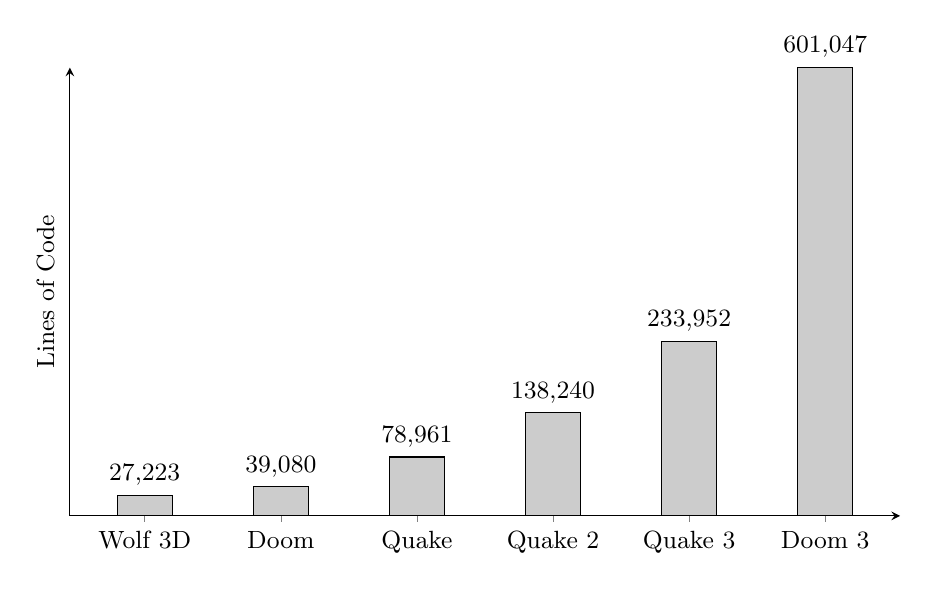
\begin{tikzpicture}[font=\small]
    \begin{axis}[
      width=\textwidth,
      height=0.6\textwidth,
      ybar=0.6\textwidth,
      bar width=20pt,
      ylabel={Lines of Code},
      ymin=0,
      ytick=\empty,
      xtick=data,
      axis x line=bottom,
      axis y line=left,
      enlarge x limits=0.11,
      symbolic x coords={Wolf 3D,Doom,Quake,Quake 2,Quake 3, Doom 3},
      xticklabel style={},
      yticklabel style={},
      nodes near coords={\pgfmathprintnumber[fixed,precision=0]\pgfplotspointmeta}
    ]
      \addplot[fill=black!20,draw=black] coordinates {
        (Wolf 3D,27223)
        (Doom,39080)
        (Quake,78961)
        (Quake 2, 138240)
        (Quake 3, 233952)
        (Doom 3, 601047)
      };
    \end{axis}
   \end{tikzpicture} 
   \caption{Line of codes from id Software game engines.}
 \end{figure}
 
\par

 \begin{fancyquotes}
   We didn't have spell checkers in our editors back then, and I always had poor spelling.  The word "collumn" appears in the source code dozens of times.  After I released the source code, one of the emails that stands out in memory read:
 \bigskip \\
It's "COLUMN", you dumb @\#\$\% !\\
 \bigskip \\
\textbf{John Carmack - Programmer}
 \end{fancyquotes}
 
The archive contains more than just \codeword{.H} (headers) and \codeword{.C} (code) files. Also present are:
\begin{itemize}
\item \codeword{GOODSTUF.TXT:} Two emails from fans demonstrating the success of the game: An ex-POW and a Microsoft employee.
\item \codeword{.ASM:} Assembly routines to optimize 3D renderer. Also contains low level routines for I/O.
\item \codeword{SIGNON.OBJ:} The startup screen showing the system characteristic (RAM, EMS, XMS, Joystick, SoundCards) was linked in the binary. The reason why is given later.
\item \codeword{GAMEPAL.OBJ:} Game palette. Hardcoded and linked in the executable for the same reason described previously.
\item \codeword{README:} How to build. You can also find a complete tutorial in the Annexe of this book.
\item Many files resulting from a previous compilation attempt.
\end{itemize}







\section{Big picture}
The engine can be divided in three blocks:
\begin{itemize}
\item The 2D renderer let the user set the game.
\item The 3D renderer where most of the time is spent in the game.
\item The sound system which always run concurrently with either 2D or 3D renderer. 
\end{itemize}
Note the three systems communicate via shared memory. The renderer issue music and sound request to the RAM (also making sure the assets are ready). The sound system also communicates with the renderers since it is in charge of the heartbeat of the whole engine. The renderer can update the world according to the wall-time tracked by \cw{TimeCount} variable.
\par
\begin{figure}[H]
\centering
 \includegraphics[width=\textwidth]{imgs/drawings/three_systems.pdf}
 \end{figure}
 \par

 









\subsection{Unrolled loop}
With the big picture in mind, we can dive into the code and unroll the main loop (\cw{int main()}) to reveals two renderers (the sound system is interrupt driven and therefore is out of \cw{main}). An important precision about data types: Because the game is using Real Mode, C types don't mean what people would expect from a 32 bits architecture.\\
\begin{itemize}
\item \cw{int} and \cw{word} are 16 bits long.
\item \cw{long} and \cw{dword} are 32 bits long.
\end{itemize}

\par
\begin{minipage}{\textwidth}
\lstinputlisting[language=C]{code/unrolled_loop_main.c}
\end{minipage}
\par

\par
In \cw{InitGame}, the engine starts up and bring up all the managers (those are described in details later):\\
\par
\begin{minipage}{\textwidth}
\lstinputlisting[language=C]{code/unrolled_loop_init.c}
\end{minipage}
\par
Then come the core loop where 2D renderer and 3D renderer are called forever:\\
\par
\begin{minipage}{\textwidth}
\lstinputlisting[language=C]{code/unrolled_loop_demoloop.c}
\end{minipage}
\par
\cw{PlayLoop} contains the 3D renderer. It is pretty standard with a get inputs, update world, render world approach:\\
\par
\begin{minipage}{\textwidth}
\lstinputlisting[language=C]{code/unrolled_loop_playloop.c}
\end{minipage}
\par
The sound system is started via the Sound Manager. It driven by Interrupt service routine 8. Notice how the ISR is tied to the PC timer and can run at at different frequency of 140, 700 or even 7000Hz depending on the needs of the sound system involved:\\
\par
\begin{minipage}{\textwidth}
\lstinputlisting[language=C]{code/soundsystem_interrupt.c}
\end{minipage}
\par

















\section{Architecture}

The engine is made of WL\_* files which rely on ID\_* sub-systems called Managers. There are seven of them in total:\\
\begin{itemize}
	\item Memory
	\item Page
	\item Video
	\item Cache
	\item Sound
	\item User
	\item Input
\end{itemize}
The WL stuff was written specifically for Wolf3D while the ID\_ managers were reused from the previous game (Catacomb 3D) and improved for the needs of the new engine.

\begin{figure}[H]
\centering
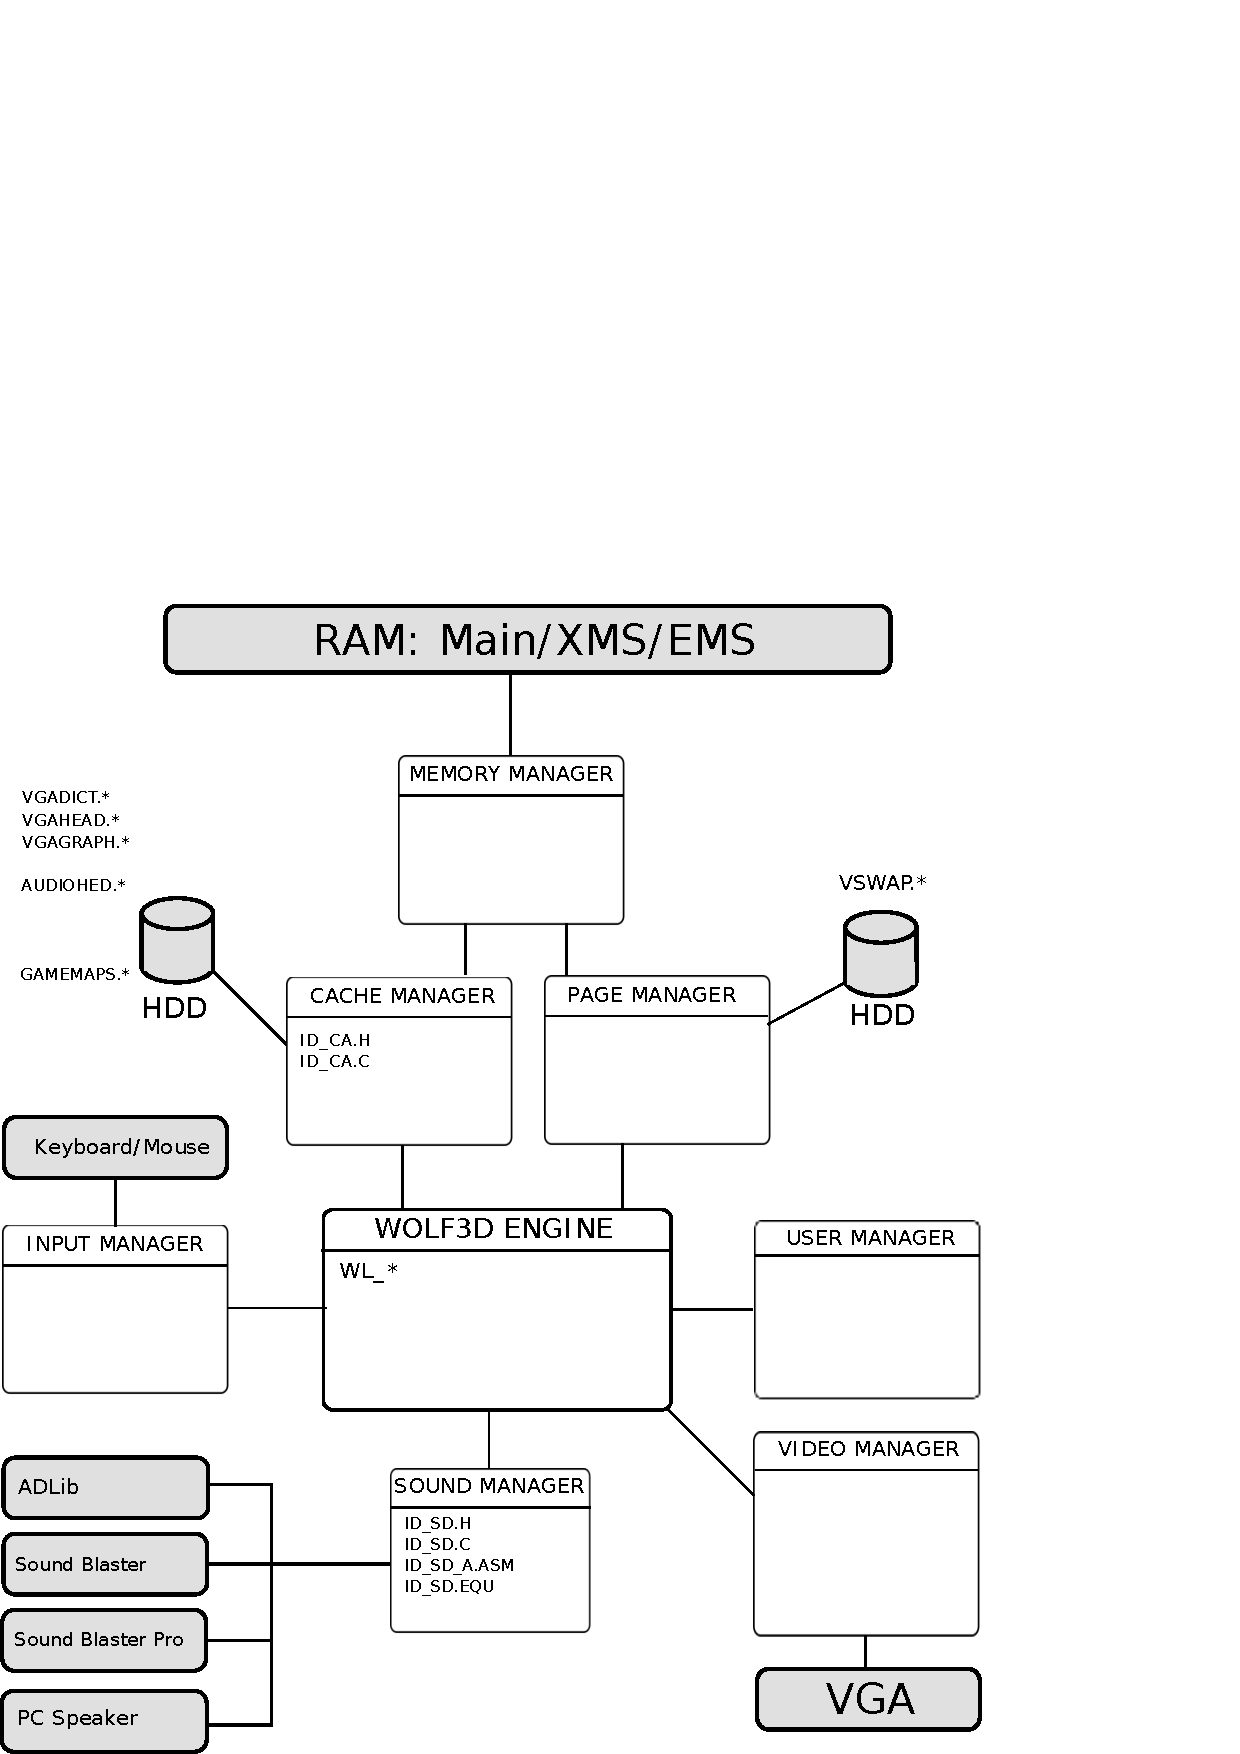
\includegraphics[width=\textwidth]{imgs/drawings/architecture.pdf}
\caption{Architecture with engine and sub-systems (in white) connected to I/O (in gray).}
\label{fig:architecture}
\end{figure}
Next to the hard drives (HDD) you can see the assets packed as described in the Team chapter.










\subsection{Memory Manager (MM)}
The engine does not rely on \cw{malloc} to manage memory because it can lead to fragmented memory and no way to compact free space. A linked list keep track of the RAM, dividing it in blocks. A block
point to a starting point in RAM and has a size:\\
 \par
\lstinputlisting[language=C]{code/mm_block.c}
 \par
A block can be marked with attributes:
\begin{itemize}
\item \cw{LOCKBIT} : This block of RAM cannot be moved during garbage collection.
\item \cw{PURGEBITS} : 0-3 level, 0= unpurgable, 3= purge first.
\end{itemize}

The memory manager starts by allocating all available RAM via \cw{malloc}/\cw{farmalloc} and creates a \cw{LOCKED} block of size 1KB at the end. The linked list uses two pointers: \cw{HEAD} and \cw{ROVER} (for the tail).
 \par
\begin{figure}[H]
\centering
 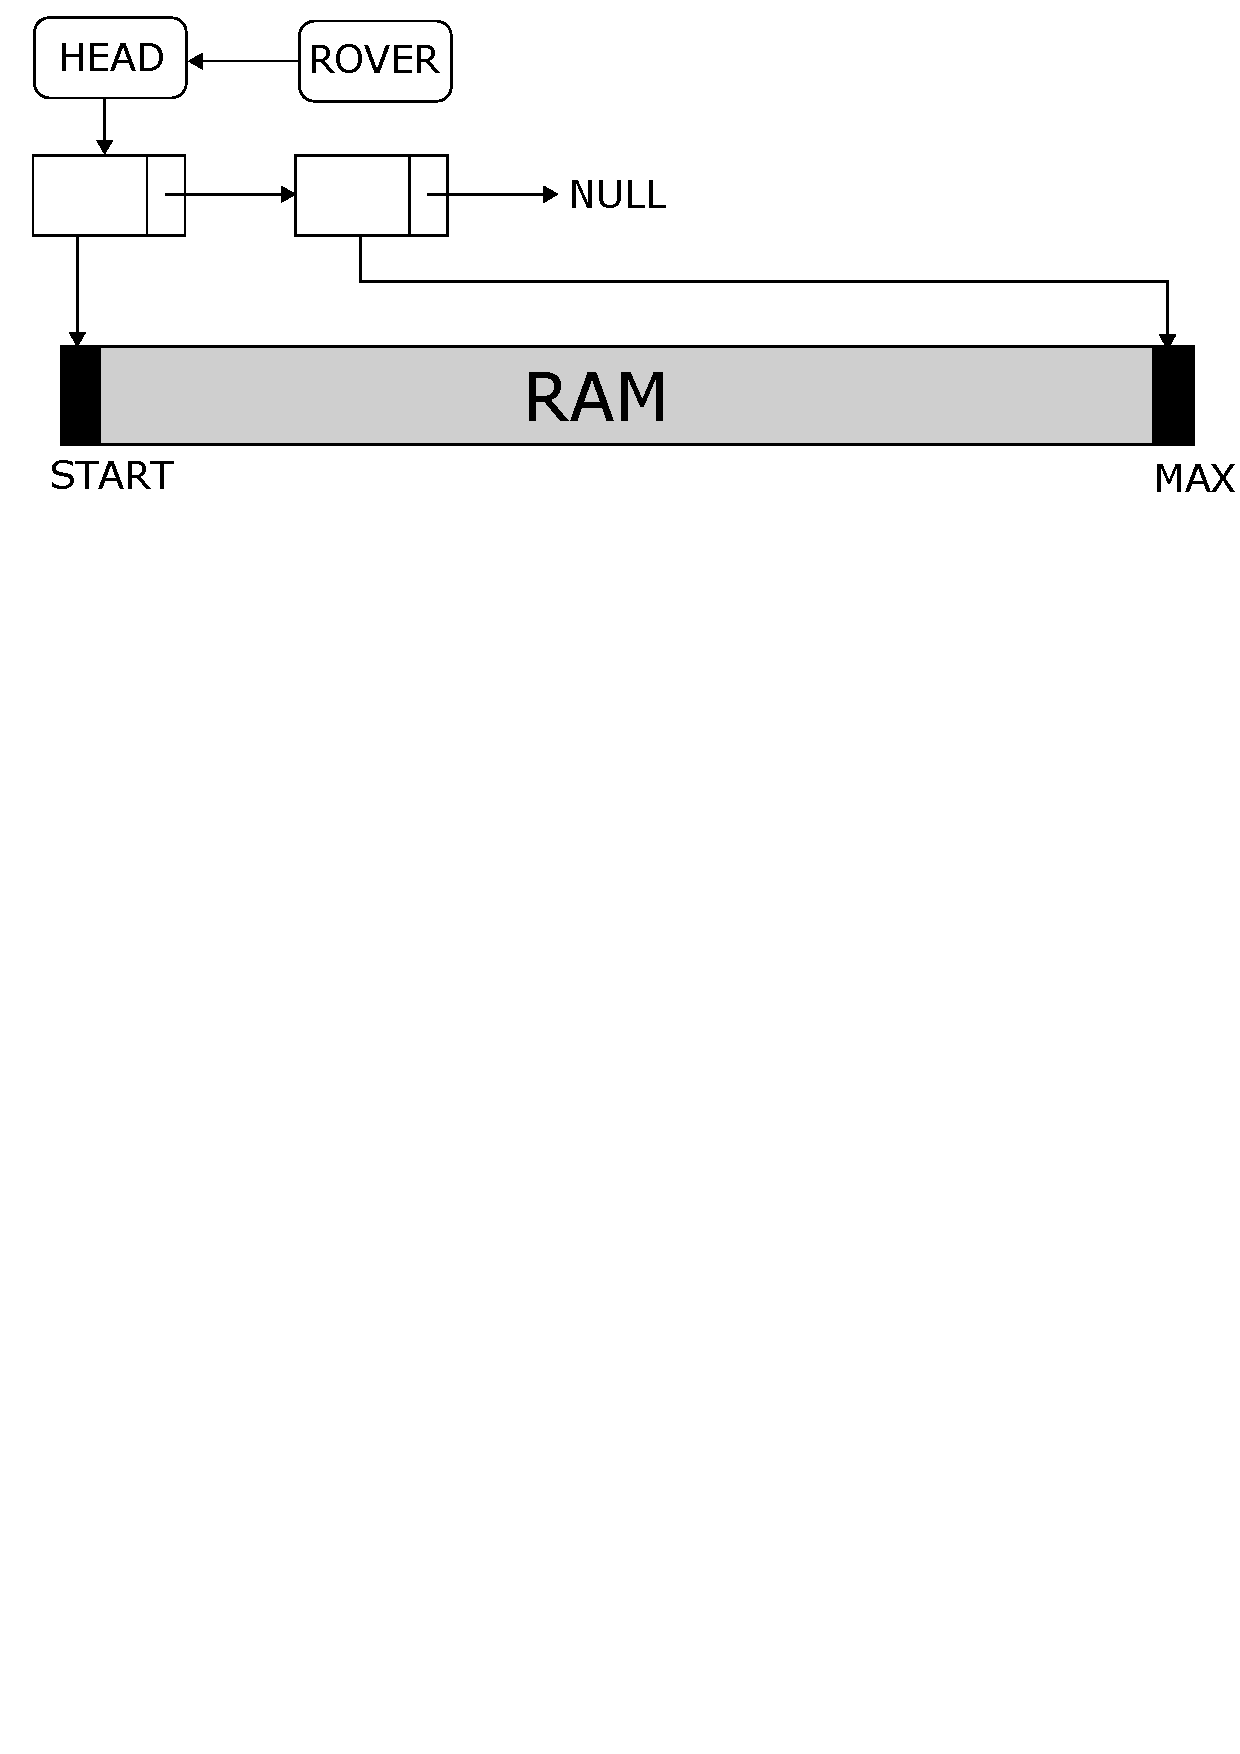
\includegraphics[width=\textwidth]{imgs/drawings/mm_start.pdf}
 \end{figure}
 \par
 The engine interacts with the Memory Manager by requesting RAM (\cw{MM\_GetPtr}) and freeing RAM (\cw{MM\_FreePtr}). To allocate ram , the manager searches for "holes" in the layout. It take up to three passes of increasing complexity:
\begin{enumerate}
\item After rover
\item After head
\item Compacting and then after rover
\end{enumerate}
\par
  The easier case is when there is enough space after the rover. A new node is added to the linked list and rover moves forward:\\
  \par
\begin{figure}[H]
\centering
 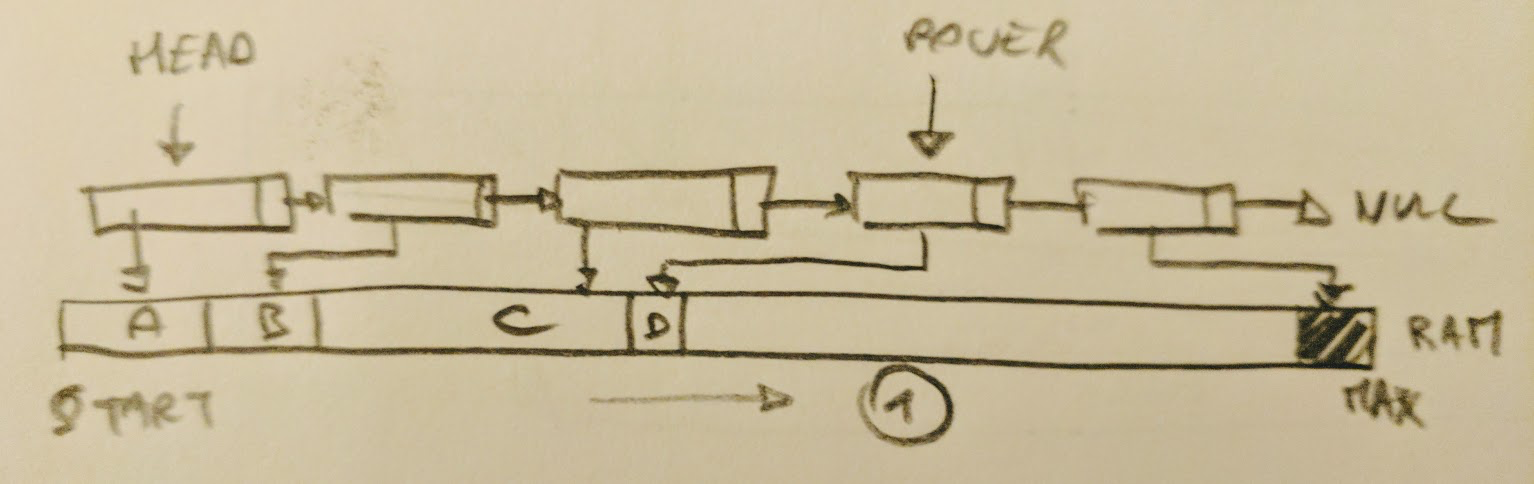
\includegraphics[width=\textwidth]{imgs/drawings/mm_after_rover.pdf}
 \end{figure}
 \par
Eventually the free RAM will be exhausted and the first pass will fail:
  \par
\begin{figure}[H]
\centering
 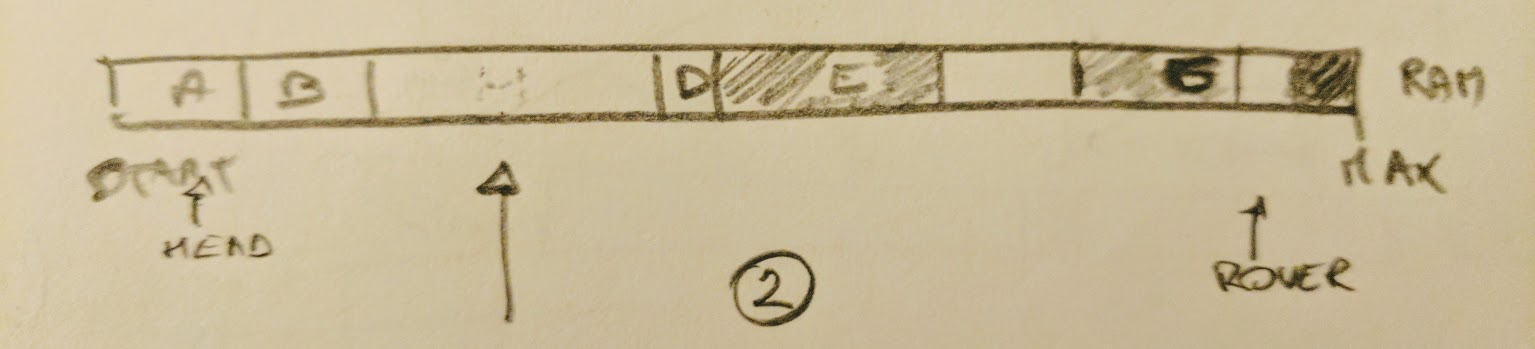
\includegraphics[width=\textwidth]{imgs/drawings/mm_before_rover.pdf}
 \end{figure}
 \par
 If the first pass fails, the second pass looks for a "hole" between the head and the rover. If for example block B was marked as \cw{PURGEABLE}, it will be deleted and replaced with the new block E and fragmentation starts to appear (like if \cw{malloc} was used):\\
 \begin{figure}[H]
\centering
 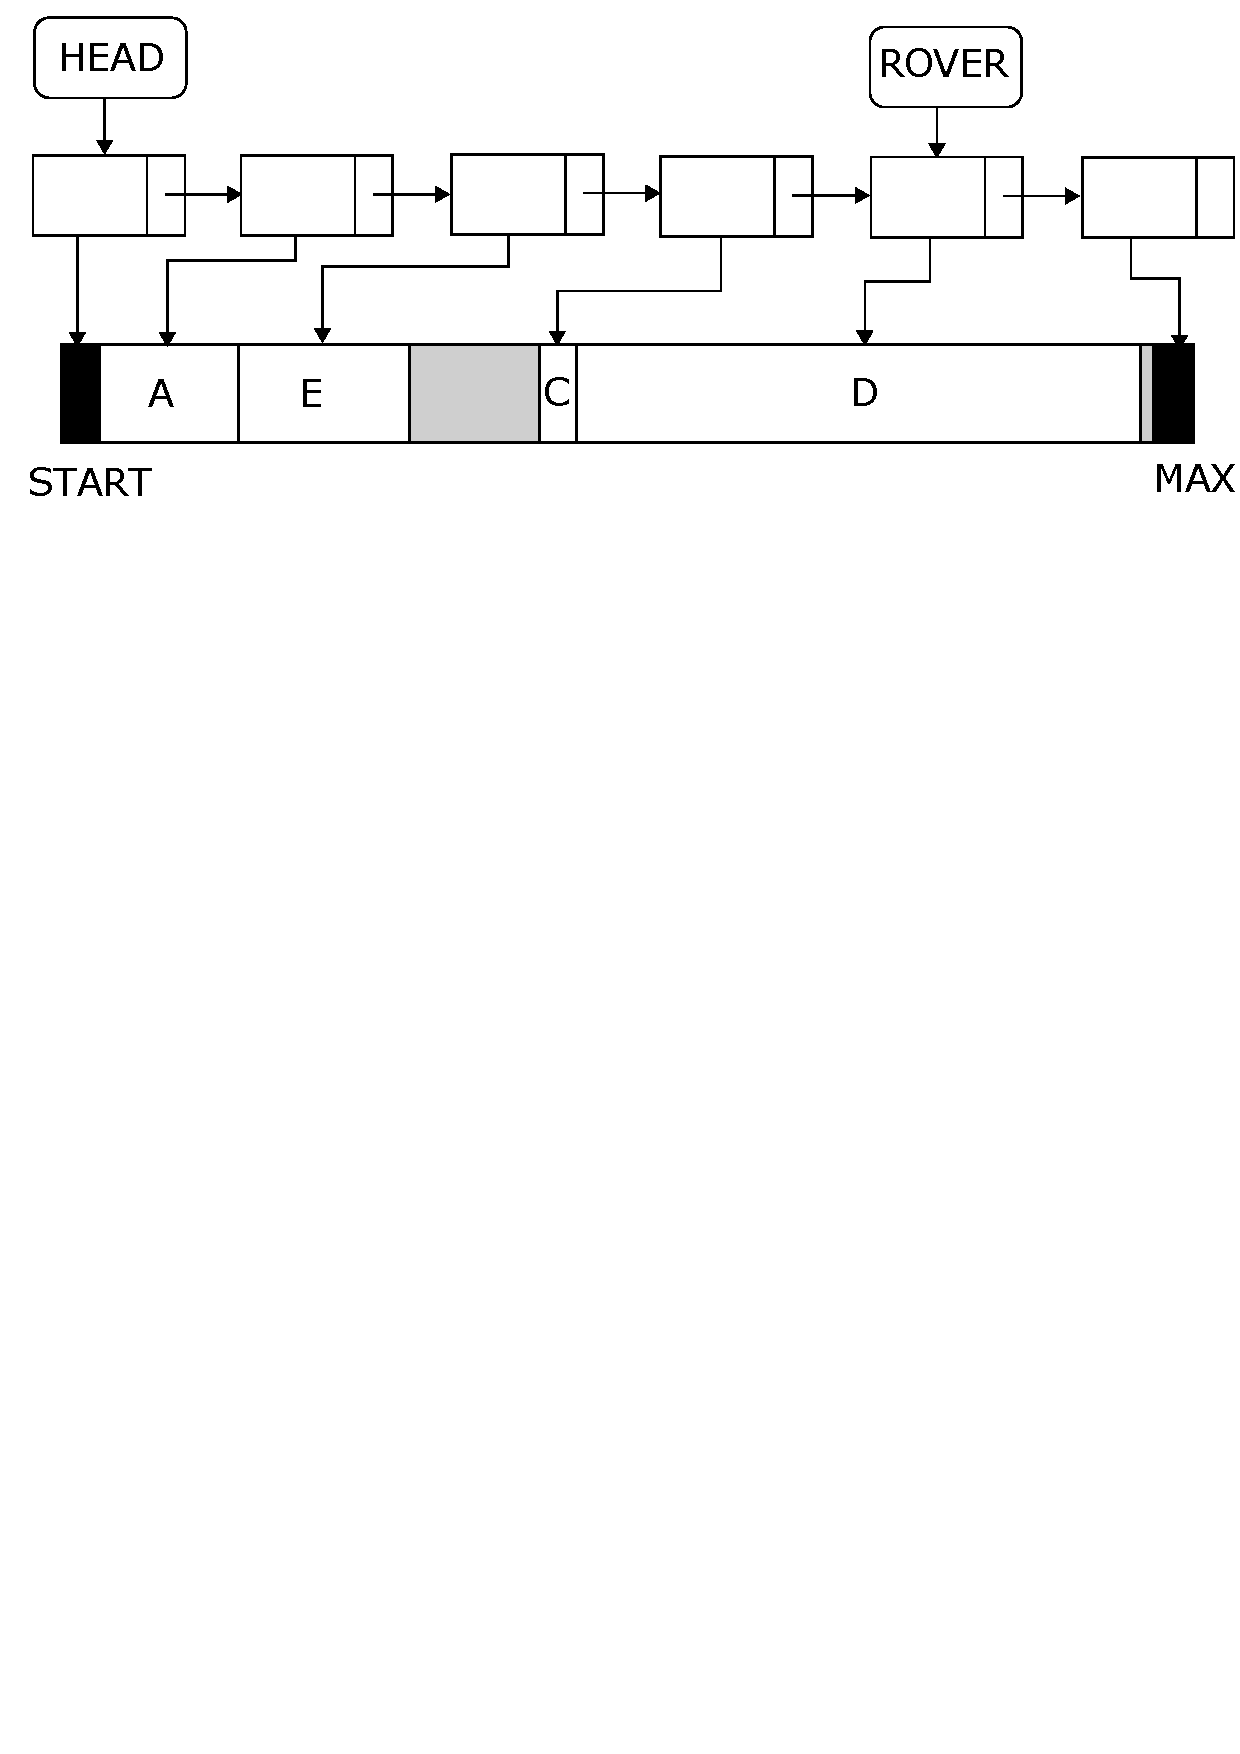
\includegraphics[width=\textwidth]{imgs/drawings/mm_after_head.pdf}
 \end{figure}
 \par
 If the RAM reaches a point where the first and second pass failed, it means there is nowhere a continuous block of memory big enough to satisfy the request. The manager is going to iterate through the entire linked list and do two things: Delete blocks marked as purgeable and compact the RAM.
  \par
\begin{figure}[H]
\centering
 \includegraphics[width=\textwidth]{imgs/drawings/mm_compact.pdf}
 \end{figure}
 \par
But if memory is moved around, how do previous allocation still point to what they had before the garbage collection phase? Notice that a \cw{mmblockstruct} has a \cw{useptr} pointer which point to the owner of a block: If it moves memory, it also updates the ower of the block.

   \par
\begin{figure}[H]
\centering
 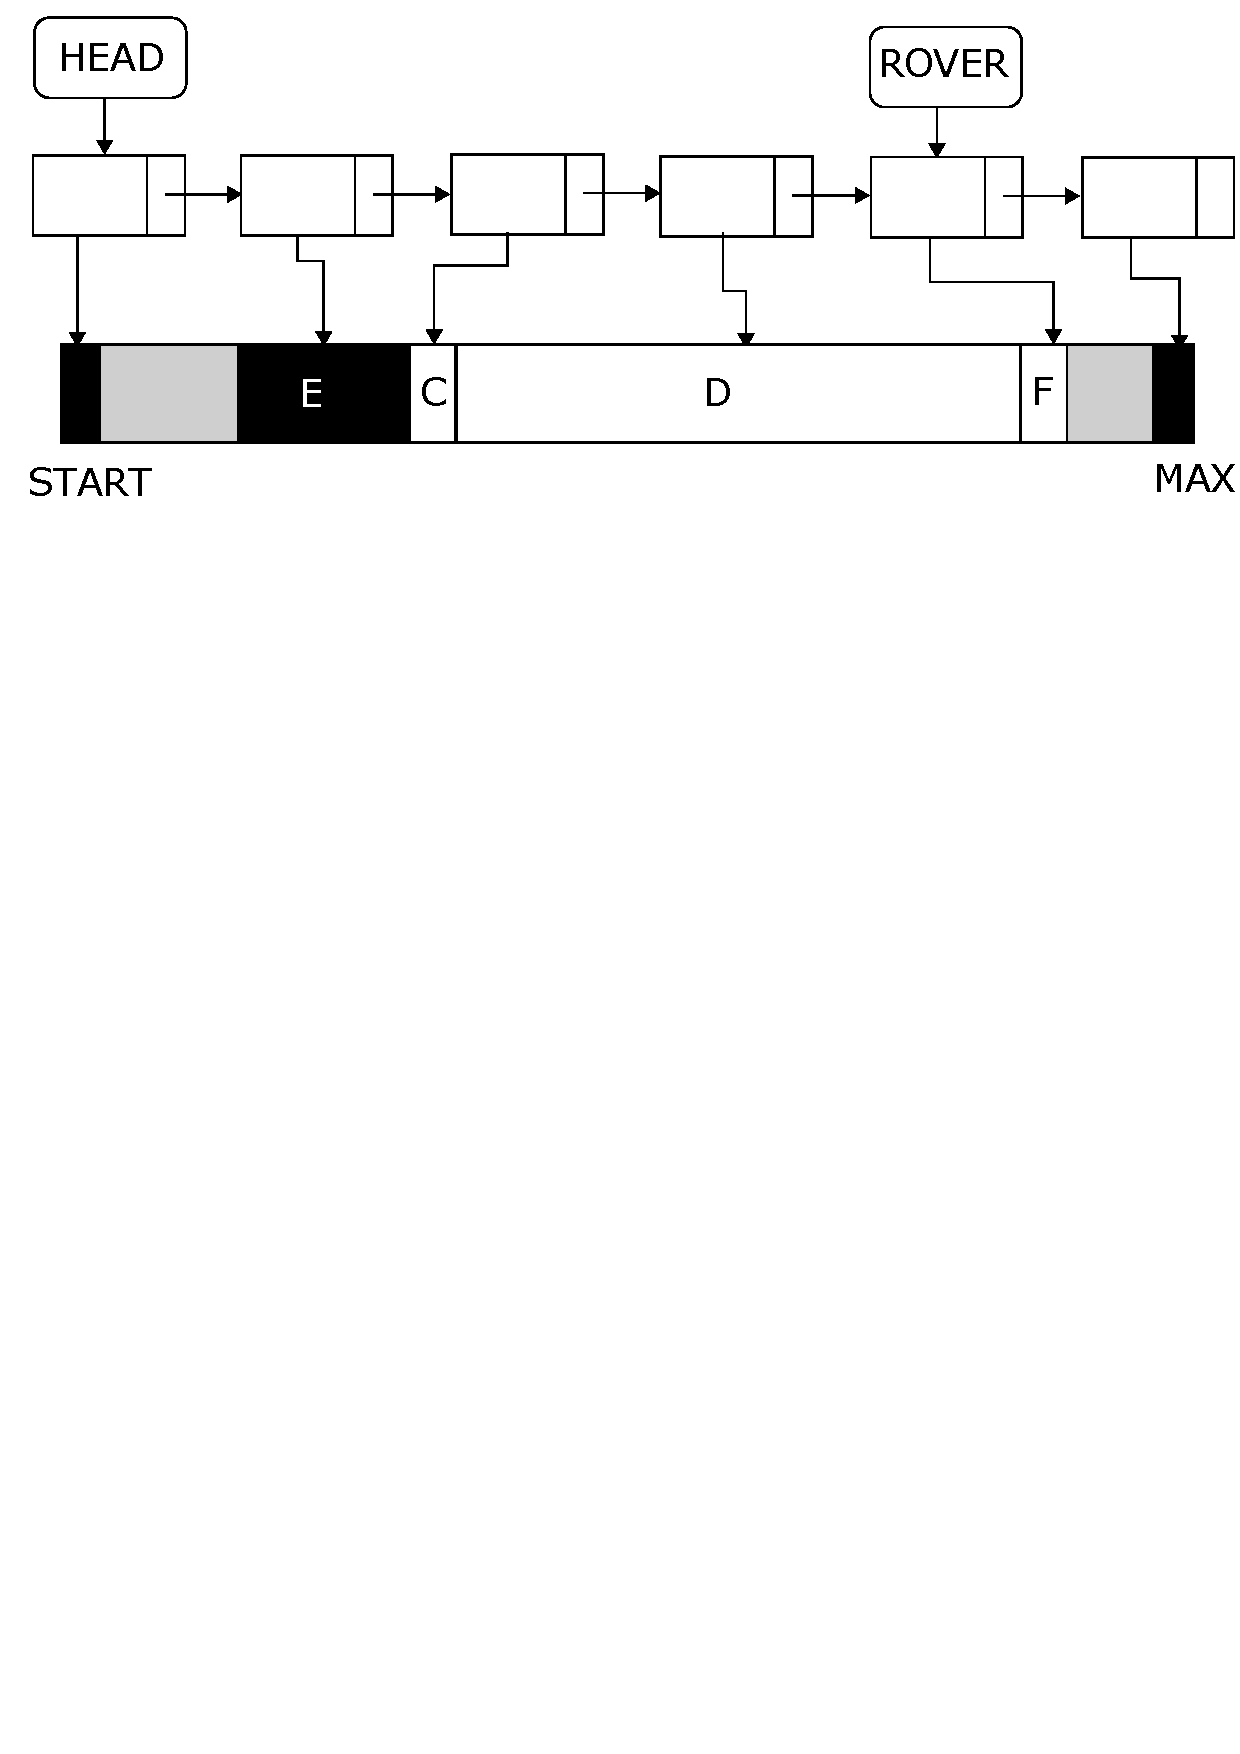
\includegraphics[width=\textwidth]{imgs/drawings/mm_bad_compact.pdf}
 \end{figure}
 \par
 Note that since some block can be marked as \cw{LOCKED}, the compacting will be disturbed: Upon encountering a locked lock, compacting start after it, even is there was space available between the last block and the locked block.












\subsection{Page Manager (PM)}
The Page Manager is dedicated to the 3D engine. Its task is to make sure assets such a wall texture, sprites and sound effect at available in RAM. Jason Blochowiak seems to be the main author and his previous experience with Unix system clearly influenced the design of this component. It is built around the idea of asset container called "Page". When the engine needs a resource, its requests a page with the resource Id to the Page Manager. To fulfill the request as fast as possible, it taps in all types of RAM: Conventional, EMS and XMS. If a page is located in conventional memory or EMS, the request is considered a cache "hit" and page is returned to caller. Otherwise the request is a cache "miss". The PM looks for the page in XMS RAM and ultimately if all failed in \cw{VSWAP.WL1} file on the HDD which contains all 3D assets.\\
 \par
\begin{figure}[H]
\centering
 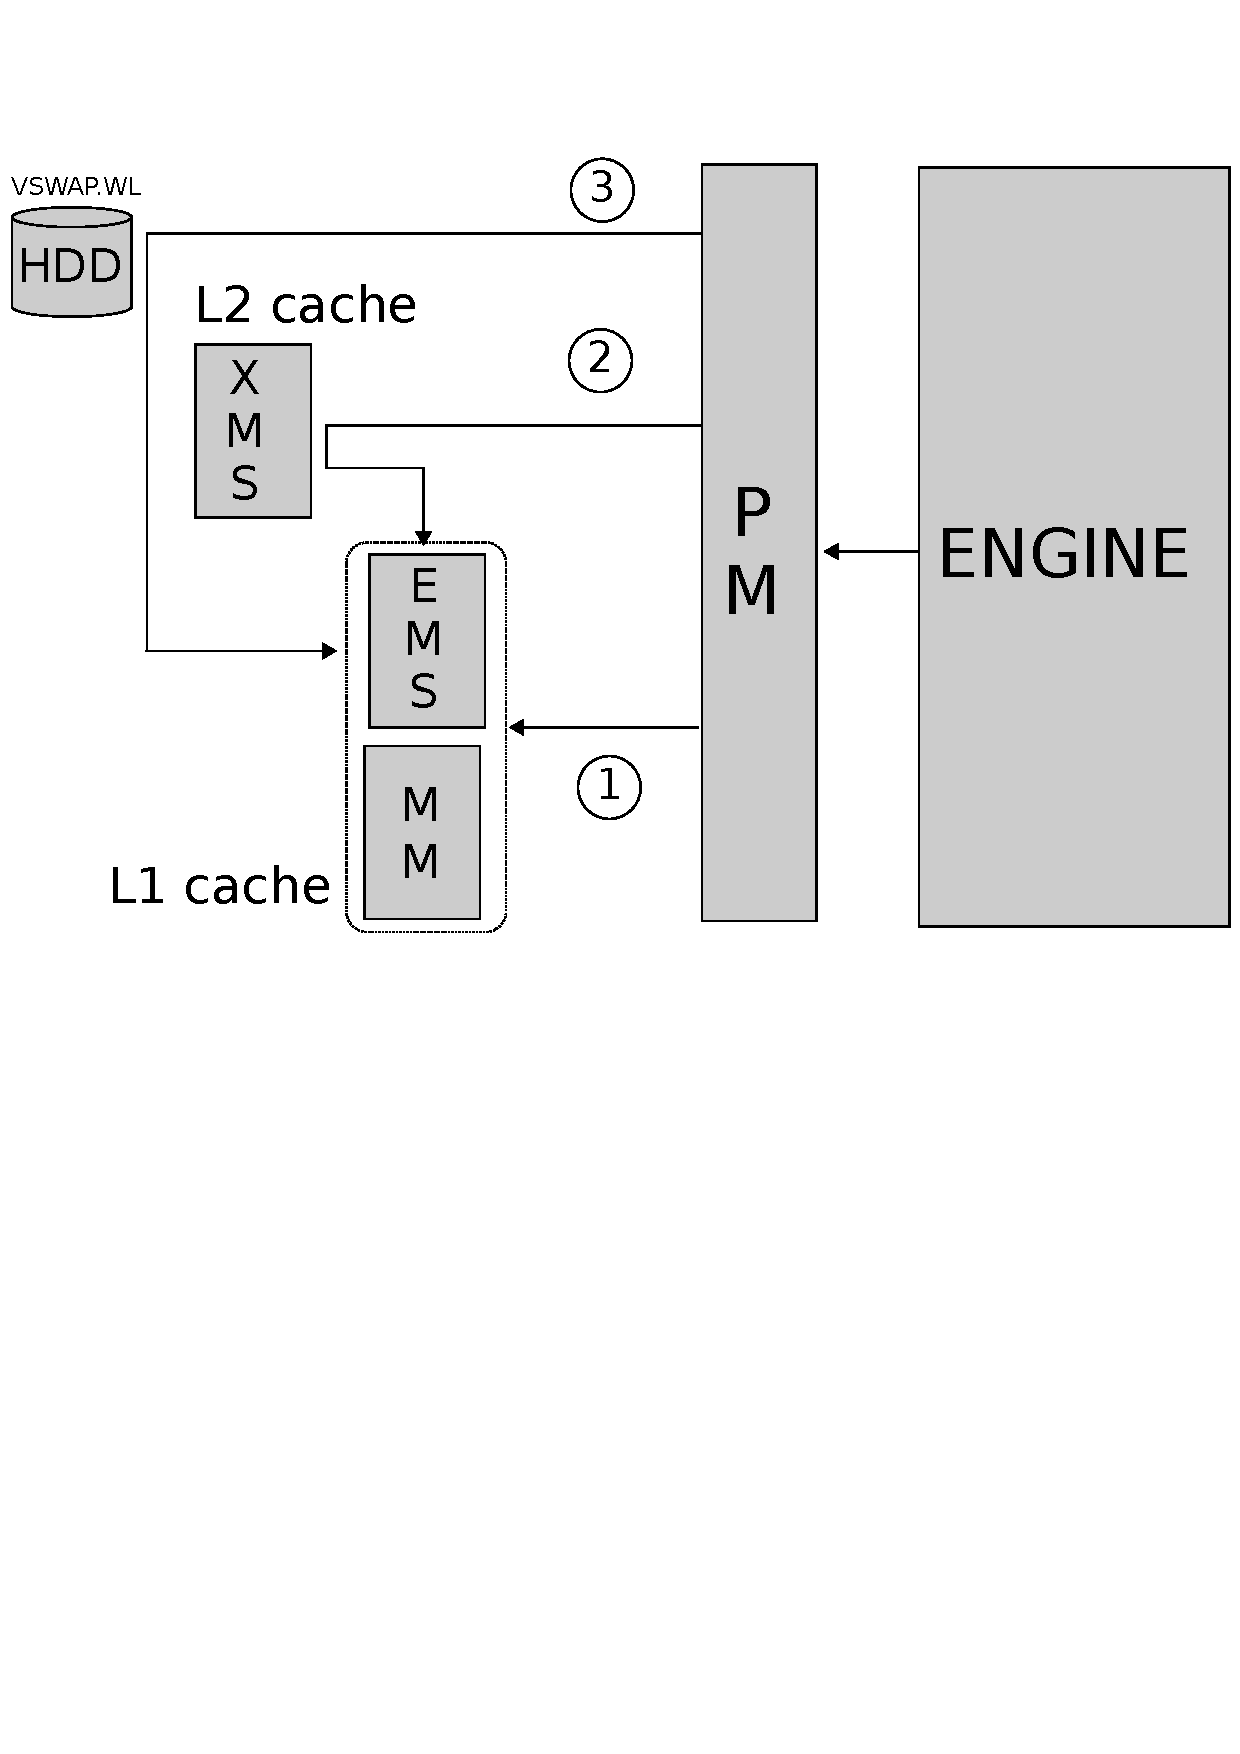
\includegraphics[width=\textwidth]{imgs/drawings/page_manager_architecture.pdf}
 \end{figure}
 \par
In order to minimize the cost of page miss, the engine preload the page cache before a level start. This is known at the "Get Psyched" screen:
 \par
\begin{figure}[H]
\centering
 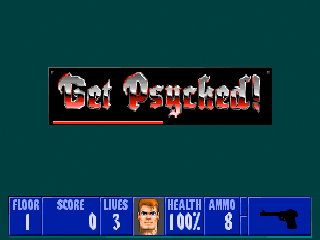
\includegraphics[width=\textwidth]{screenshots/get_psyched.png}
 \end{figure}
 \par
The precaching mechanism is not particularly clever: It loads as many page from the swap file as possible. It doesn't try to look at what is actually used in the level. But the eviction policy (LRU) ultimately stabilize the cache and even a machine with only 1MB of RAM is able to play a level with no HDD access after a few minutes. This design had a small annoying flow: On a low memory machine a cache miss would occur at the worse possible moment: When the player opens the last door and is about to find himself confronted to the heavy powered final boss, the cache manager would not have the sprites available. This would incur a HDD access, a lag and an unfair death.\\
\par
The size of the swap file varies depending on the version of the game you play: \cw{VSWAP.WL1} (shareware) is 742KB while \cw{VSWAP.WL6} (full version) is 1,500KB. In both case a machine with 2MB of RAM on top of the factory issued 1MB is enough to have all assets loaded during pre-caching.\\
\par
TODO: Insert code sample to show what an ID is.
\par
\bu{Trivia:} In the code, the progress bar was called a "thermometer".\\
\par
\bu{Trashing:} When the system has to evict pages but ends up reloading the same resource during the same frame, it is trashing. The HDD is put to heavy contribution and the framerate drops. Trashing can happen if two many different resources are visible on the screen. In order to help designers balance their creativity with the needs for a decent framerate, the engine detects trashing and flashes the screen border red when it occurs.\\
\par
\bu{Sounds are special:} Because the sound cards are fed via a system of interrupt, the sound manager cannot recover from a page miss. Therefore all sound resources are loaded first (they are located at the start of \cw{SWAP.WL1}) and they are also only loaded in Conventional memory.











\subsection{Video Manager (VL \& VH)}
The video manager features two parts:
\begin{itemize}
\item A part dedicated to VGA register manipulation.
\item A part dedicated to 2D menu drawings.
\end{itemize}
\par
This part features what I think is one of the most beautiful trick in the game: FizzleFade which is explained later.






\subsection{Cache Manager (CA)}
A small manager performing a lot: Interface with map, graphic and music. Assets are stored in two files: One header file performing the translation between resource ID and offset in the DATA file and an other file containing he actually payload.\\
 \par
\begin{figure}[H]
\centering
 \includegraphics[width=\textwidth]{imgs/drawings/cache_manager_architecture.pdf}
 \end{figure}
 \par
\bu{Note:} All resources are compressed. The CM handle decompression transparently.
\begin{verbatim}
http://www.shikadi.net/moddingwiki/GameMaps_Format
\end{verbatim}
\bu{Trivia :} Is it a typo with filename \cw{AUDIOHEA.WL} ? Correct spelling would be \cw{AUDIOHEAD.WL}. Where is the \cw{D}? This is in fact a limition of the operatin system. DOS 5 only allows 8.3 filename (at most eight characters followed by at dot and at most three character for the extension).








\subsection{User Manager (US)}
\begin{minipage}{0.7\textwidth}
Largely based on Catacom 3D code and written by Jason Blochowiak. The copy/past is very visible since 90\% of the functions declared in the header (ID\_US.H) are not actually implemented in \cw{ID\_US.C}. 
It is a poorly named manager since it takes care mostly of graphic layout. When a \cw{WL\_*} high level routines needs to draw a string, it is passed to \cw{US\_Print} which does all measurement (e.g: Draw string centered)
and then passes these information to the Video Manager (\cw{VW\_DrawPropString}) which takes care of rendition.
\end{minipage}
\begin{minipage}{0.3\textwidth}
\begin{flushright}
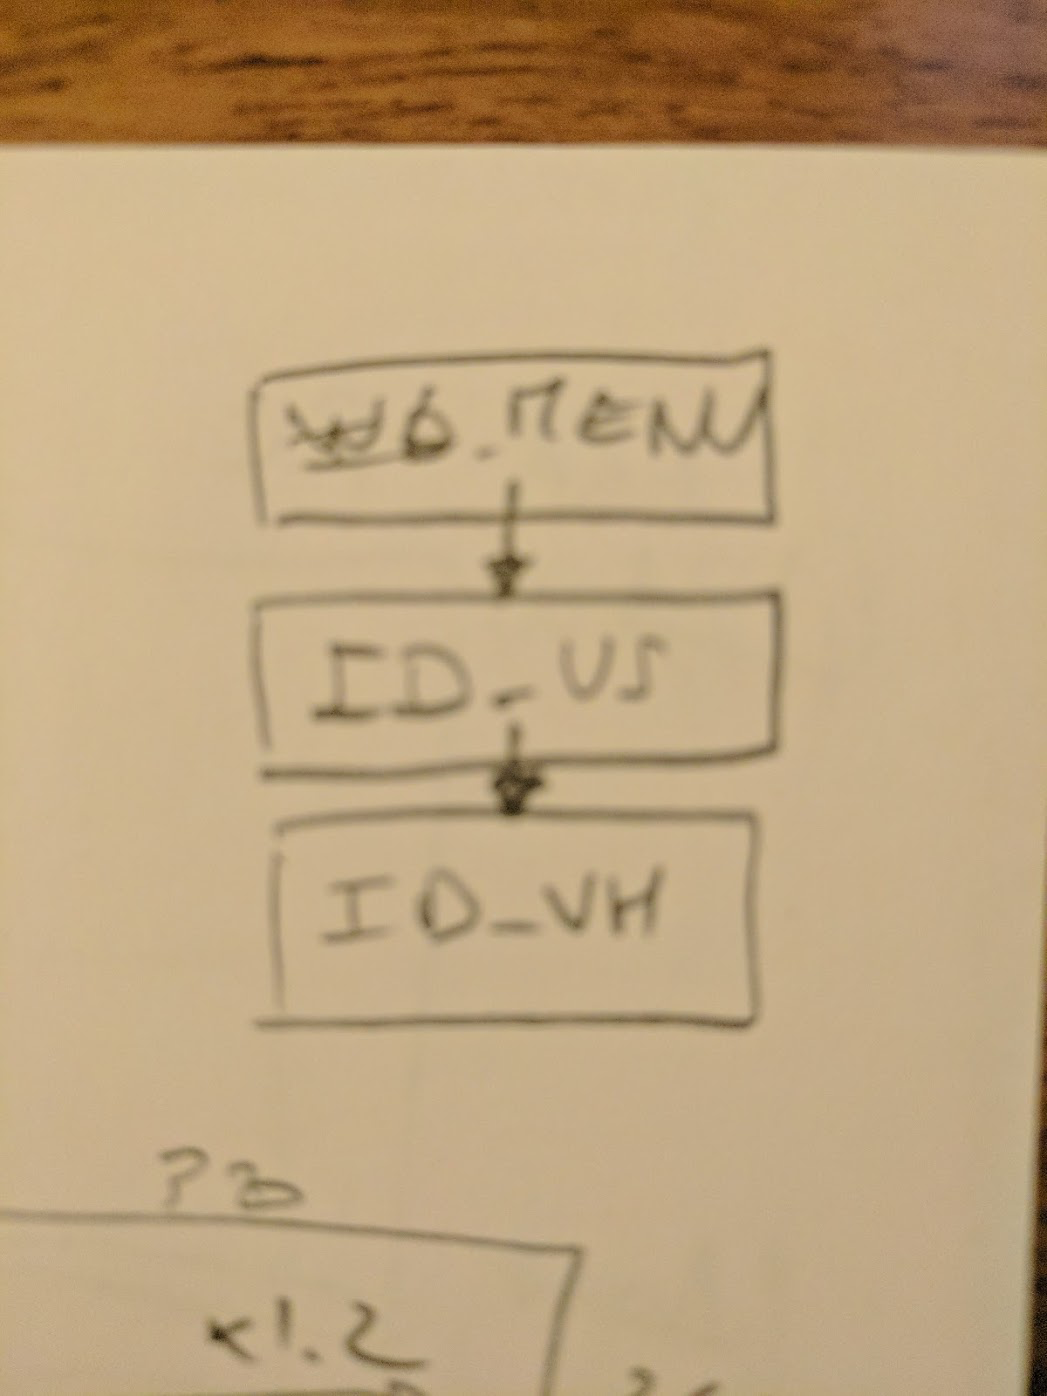
\includegraphics[width=0.8\textwidth]{imgs/drawings/US_explained.png}
\end{flushright}
\end{minipage}
\noindent
\\












\subsection{Sound Manager (SD)}
The Sound Manager abstracts interaction with all four sound systems supported: PC Speaker, ADLib (Music only), Sound Blaster and SoundSource. It is a beast of his own since it doesn't run inside the engine. Instead it called via IRQ at a much higher frequency than that engine (the engine runs at 70Hz, the sound manager ranges from 150Hz to 7000Hz). For efficiency it is written in assembly and is privileged when it comes to memory allocation: All its allocation are in Conventional Memory and its assets can never miss the cache in the Page Manager.\\
 \par
\begin{figure}[H]
\centering
 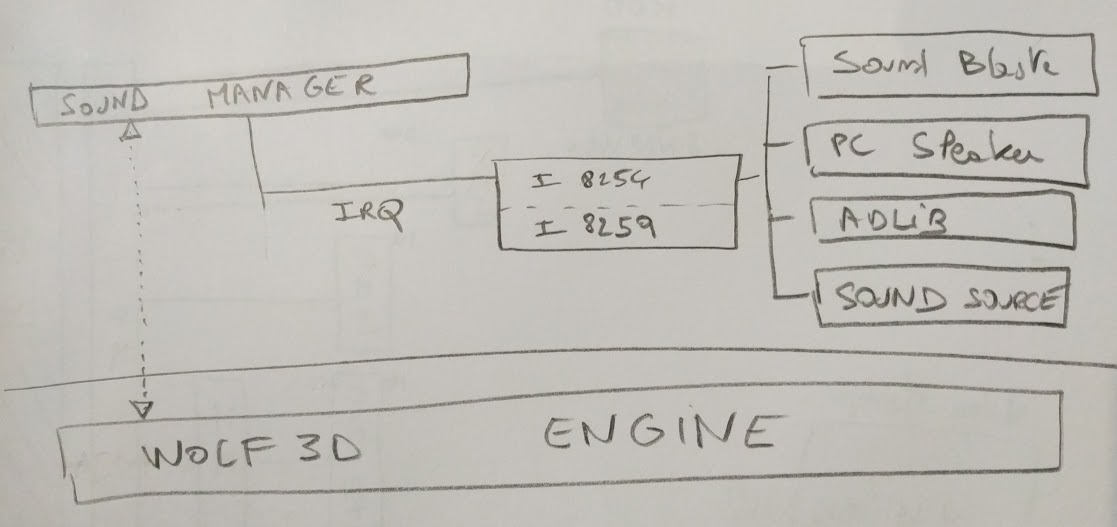
\includegraphics[width=\textwidth]{imgs/drawings/sound_manager_architecture.pdf}
 \end{figure}
 \par
The sound manager is described extensively in the "Sound and Music" section.

















\subsection{Input Manager (IN)}
Abstract interaction with joystick keyboard and mouse. Features a lot of boring boilerplate code to deal with PS/2, Serial and DA-15 ports.
















\section{Startup}
As the game engine starts, it deals with difficulties showed in the hardware section. This is where things become really interesting.

\subsection{Signon}
Tne first (mild) issue to deal with is the heterogenous ecosystem of PCs on the market. With different drivers loaded and different sound cards, the engine has to figure out how much RAM is installed and if it will be able to run. If not it has to let the user know what is the problem. That was important since id Software was a small team and they did not have CSR around to pickup the phone.\\
\par
That is what the "signon" screen is for. Note how the screen and palette are just variable, already load in RAM by the operating system. After usage \cw{signon} is unloadede from RAM to make space for the actuall game.\\
\par
\begin{figure}[H]
\centering
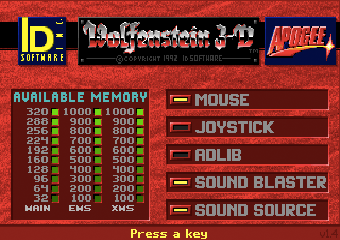
\includegraphics[width=\textwidth]{screenshots/signon.png}
\caption{Architecture and sub-systems.}
\end{figure}
\par


\par 
\begin{minipage}{\textwidth}
\lstinputlisting[language=C]{code/signonscreen.c}
\end{minipage}
Since this screen is showed almost before anything else is initialized (video system, cache manager interfacing with HDD) the full 64K images (along with the pallete) is linked against the executable. The engine only has copies from RAM to the VGA banks.\\
\par
\note{Why only show the RAM only up to 320KB? Did the game ran on 320?}
%Notice the main RAM (conventional memory) which goes only up to 320K: Between the executable and other residence routines it is all what was remaining of the original 640K. The game is able to run on 320KB but you needs to swap with the HDD at runtime to load textures and sprites.




















\subsection{Solving the VGA problem}
The Hardware chapter describing the video system left us with an unsolved problem: All of the VGA modes lack double buffering capability.\\
\par
 The most appealing mode (13h) offers a single framebuffer at a resolution of 320x200 non-square pixels with 256 indexed colors. The Chain-4 chipset in the VGA circuitry automatically maps the RAM starting at \cw{A000:0000} to the four VRAM banks. 
 \par
 \begin{figure}[H]
\centering
      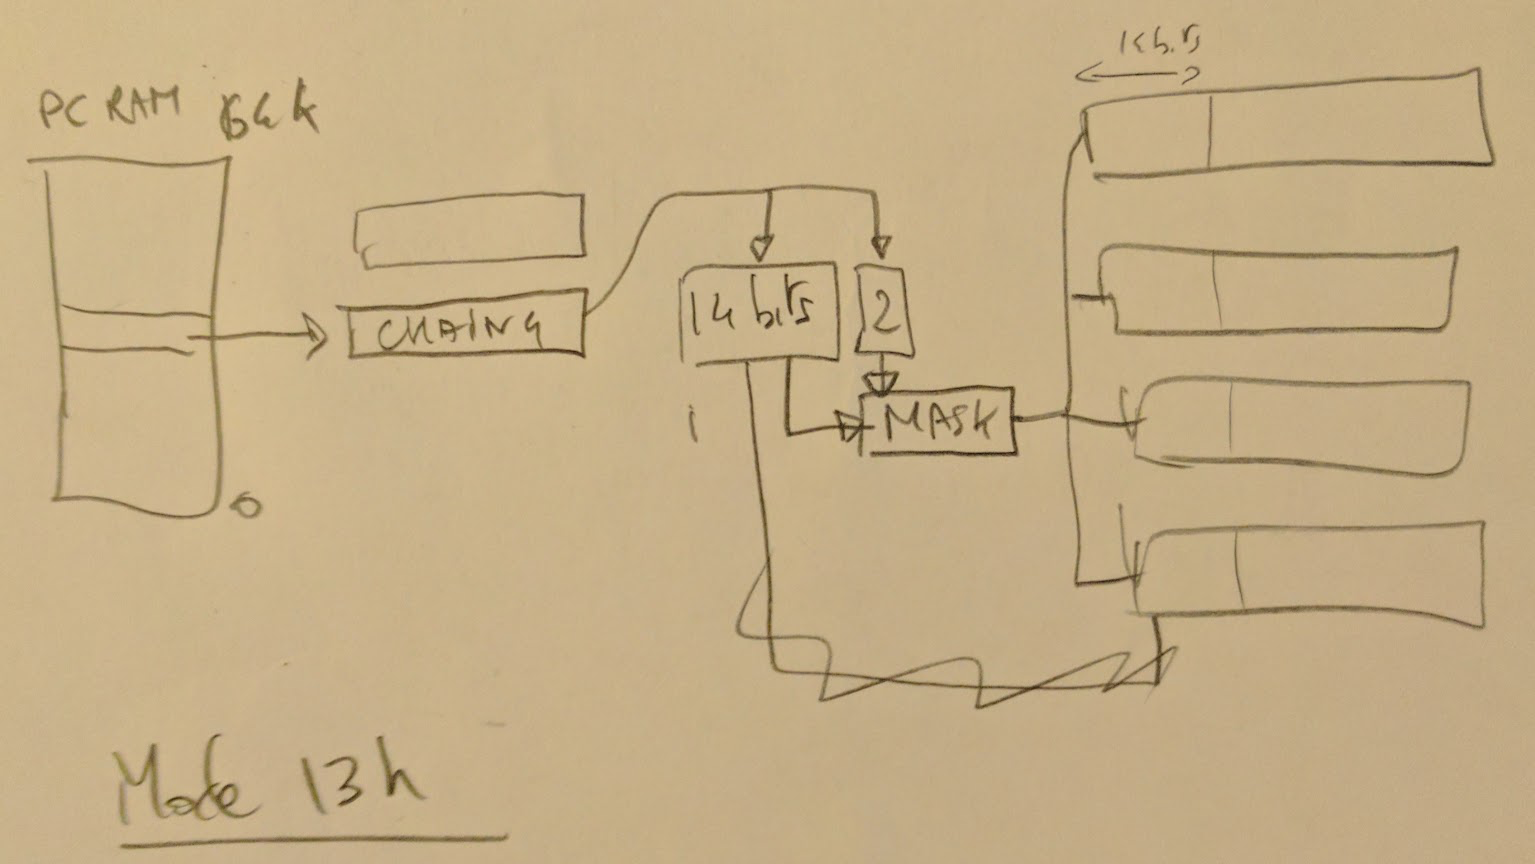
\includegraphics[width=\textwidth]{imgs/drawings/mode_13h.pdf}
\end{figure}

It is called "chaining" and because 2 bits out of the address are used to route a write/read operation to a bank, only 14 bits are used for the actuall offset in the bank. Since 14 bits can address 16384 values this system results in a waste of 75\% of the RAM to offers.\\

\begin{figure}[H]
\centering
 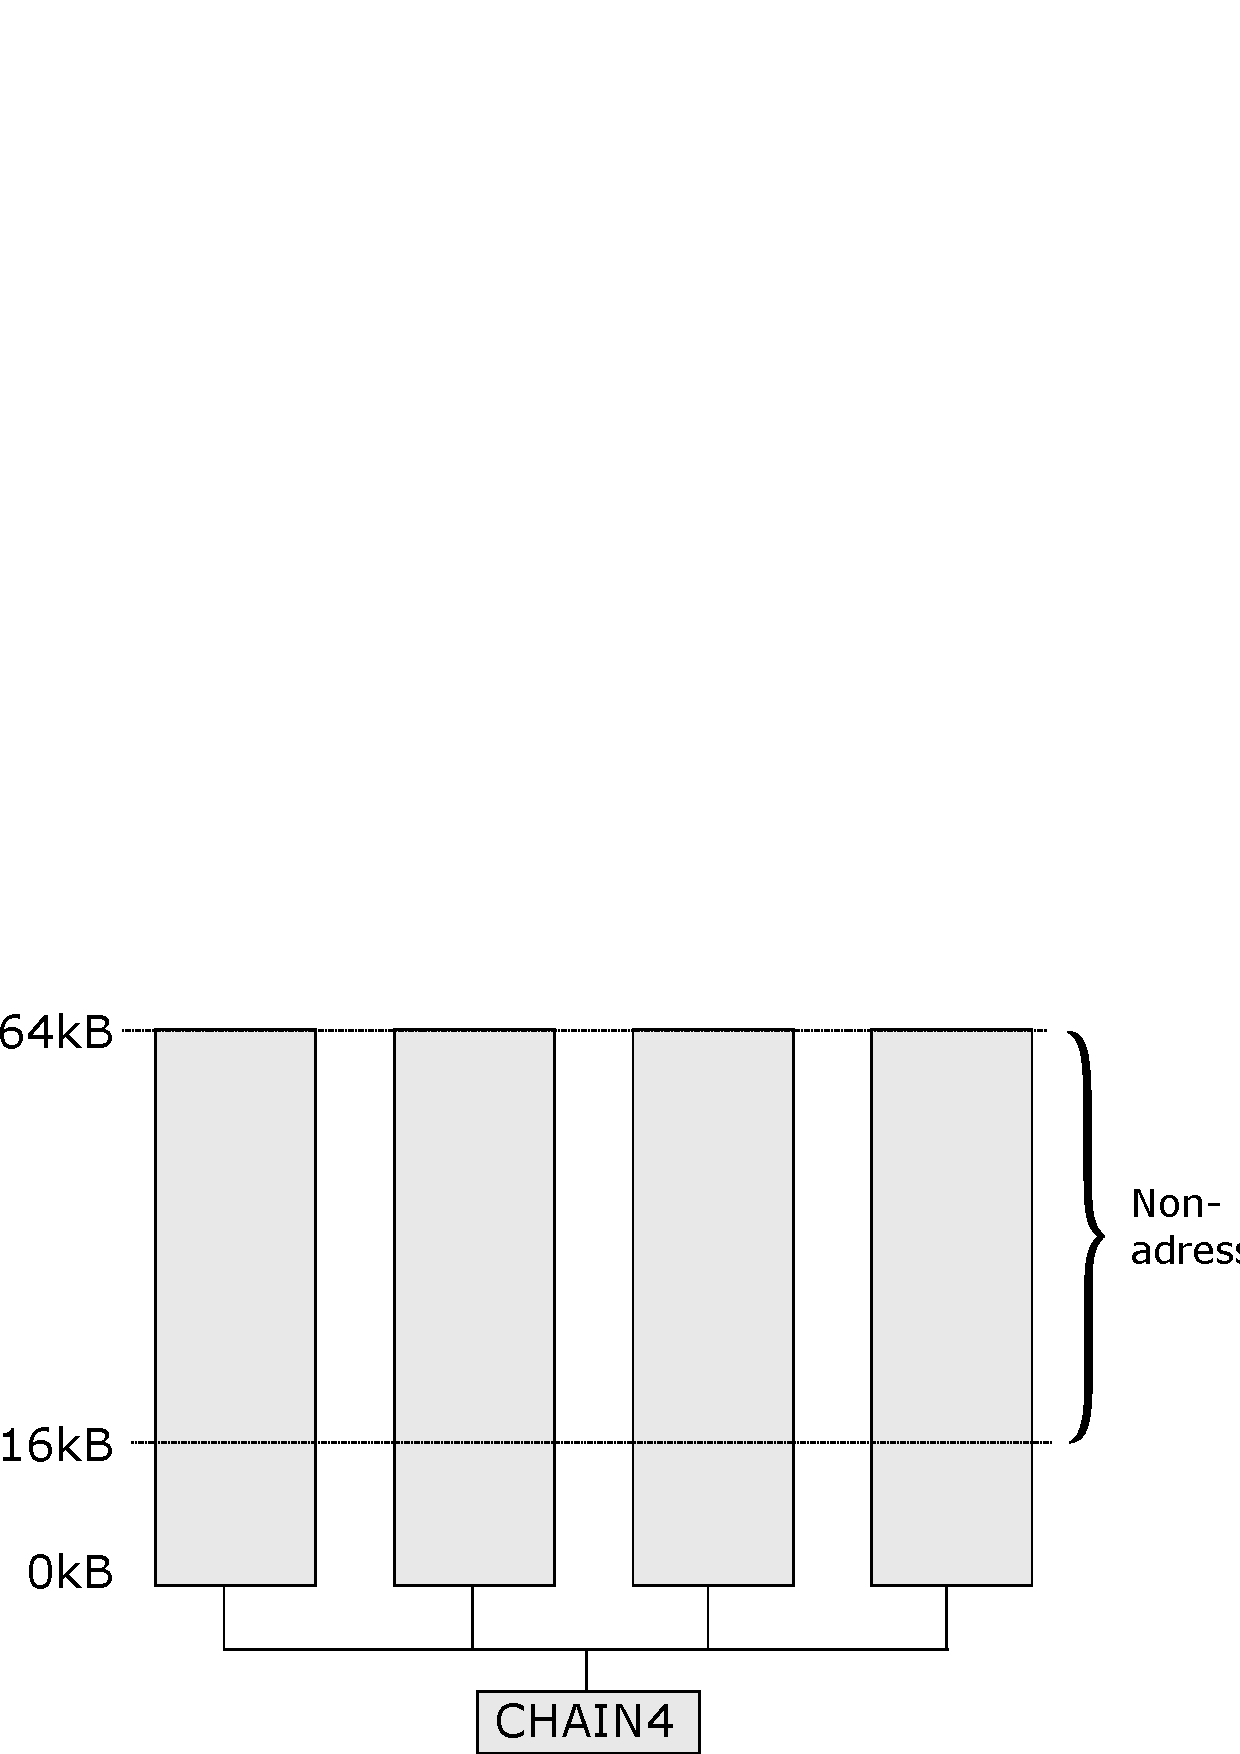
\includegraphics[width=\textwidth]{imgs/drawings/vga_layout/wasted_vga_ram.pdf}
 \end{figure}

 \par
 The problem really is the Chain-4 chip. Nobody can remember who discovered first but the process to disable it was popularized by Michael Abrash\footnote{in Dr. Dobb's Journal} in July 1991. In his article he described was he called the Mode-X. An undocumented mode with a resolution of 320x240 allowing up to four buffers in VRAM.\\
 \par
 Wolfenstein 3D does things slightly differently. It disables chain-4 but says in resolution 320x200. This mode is known as Mode-Y:\\
\note{Why not use mode X. It offered square pixels ???!}
\note{Ask John Carmack why they went for Mode-Y instead of Mode-X which offered square pixels.}
 \par
  \begin{minipage}{\textwidth}
\lstinputlisting[language=C]{code/init_vga.c}
\end{minipage}
 \par

The real magic is in function \cw{VL\_DePlaneVGA}:\\

 \par
 \begin{minipage}{\textwidth}
\lstinputlisting[language=C]{code/unchaining.c}
\end{minipage}
\note{What is long mode? What is byte mode?}
 \par
 With that much RAM available, the VRAM is divided in four parts.:
 \begin{itemize}\label{SetupPages}
 \item 64K for Framebuffer 0
 \item 64K for Framebuffer 1
 \item 64K for Framebuffer 2
 \item 64K for Graphic assets
\end{itemize}
\par
\begin{figure}[H]
\centering
 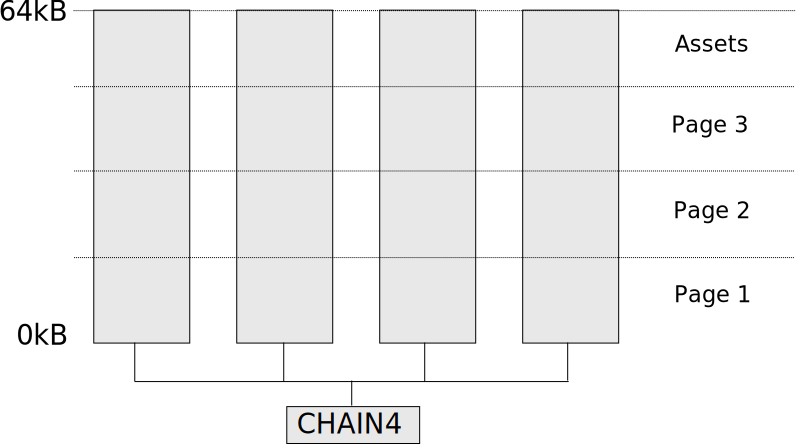
\includegraphics[width=\textwidth]{imgs/drawings/vga_layout/vga_ram_architecture.pdf}
 \caption{3D View as is appears on screen} \label{fig:vga_layout_in_3D}
 \end{figure}
\par
But the engine is not done yet. Tweaking Mode 13h into Mode-Y solves one big problem but introduced two new ones. One is about speed and the other is about correctness.\\
\par
Let's look at speed first. With chain-4 out of the picture a developer is now in charge of selecting the bank to write to. This can easily be done with a simple function:\\
\par
 \par
 \begin{minipage}{\textwidth}
\lstinputlisting[language=C]{code/select_plan.c}
\end{minipage}
 \par

Now the code sample from the hardware chapter to clear the screen become:\\
\par
\par
\begin{minipage}{\textwidth}
\lstinputlisting[language=C]{code/cleanScreenNaive.c}
\end{minipage}
\par
The code looks innocuous...but as simple as it is, it cannot run at more than 5 frames per second. The problem is that we replaced something done in hardware with something done in software: the \cw{outp} instructions which are slow.\\
\par
The solution is to change how we draw onto the screen. Instead of going top to bottom and left to right, we need to go left to right and top to bottom which minimize the number of bank switch.

\begin{minipage}{\textwidth}
\lstinputlisting[language=C]{code/cleanScreenClever.c}
\end{minipage}

\par
This code can run without issues at 70 frames per second: Only 200 slow out instruction are used.\\
\par
This speed consideration has a fundamental impact on the engine: To draw anything fast, it has to be drawn \underline{vertically}. So everything in the engine is drawn this way: Walls, Sprites, Menu. Everything. The ramification of this hardware constraint are felt everywhere. From the way assets are stored (rotated 90 degres) and compressed.. In Wolfenstein 3D: Everything has to be vertical!\\

\par
The second issue introduced by Mode-Y is about correctness. With three pages available, the engine draws in page 1, then page 2, then page 3 and then goes back to page 1 (notice there are three buffers but this is not triple-buffering). It never stops. It just instructs the CRT Controller that it should scan the framebuffer at a different offset after the next vsync.\\
\par
The CRT Controller start scan offset is a 16 bits value which is updated with a little bit of assembly. The code would look as follow:\\
\par
\begin{minipage}{\textwidth}
\lstinputlisting[language={[x86masm]Assembler}]{code/pageflip.c}
\end{minipage}
This code looks like it would work. But there is a major flaw with it. If you were to run it, every once in a while the expected screen :\\
\par
 \begin{figure}[H]
\centering
 \fullimage{full_screen.png}
 \end{figure}
Would instead appear like that:\\
\par
 \begin{figure}[H]
\centering
 \fullimage{crtc_scanstart_problem.png}
 \end{figure}
\par
Showing part of one page and a part of an other page. The framebuffer is also mis-aligned. The problem has to do with atomicity. Updating the CRTC starting address is a 16-bits value...but the \cw{out} instruction can only write 8-bits at a time. So if the pages are setup one after an other like this:
\par
\begin{figure}[H]
 \centering
 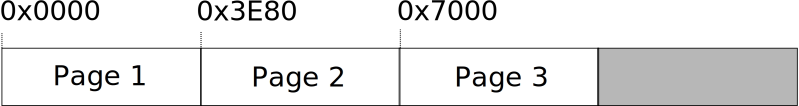
\includegraphics[width=\textwidth]{imgs/drawings/triple_pages_trick.pdf}
\end{figure}
\par
Page 0 is at 0x0000, page 1 at 0x3E80 and page 2 at 0x7000. Moving from page 0 to 1 requires updating the high byte 0x00 to 0x3E and the low byte 0x00 to 0x80. Since update is not atomic, given a poor timing the CRTC could pickup a value of 0x3E00 instead of 0x3E80:\\
\par
\par
\begin{minipage}{\textwidth}
\lstinputlisting[language={[x86masm]Assembler}]{code/pageflip_error.c}
\end{minipage}
\par
How do you update atomically a 2 bytes value with 1 byte operation? Take a look at how Wolfenstein setup its pages:\\
\par
\begin{minipage}{\textwidth}
\begin{flushright}
\lstinputlisting[language=C]{code/vga_setup_pages.c}
\end{flushright}
\end{minipage}
\par
Notice how it uses a value of 208 instead of 200 pixels for the height? That doesn't make sense at first sight. I thought it was a typo (after all 0 and 8 are visually close). The trick is to use a little bit of padding after each page so the addresses only differ by their high byte value.


\par
\begin{figure}[H]
 \centering
 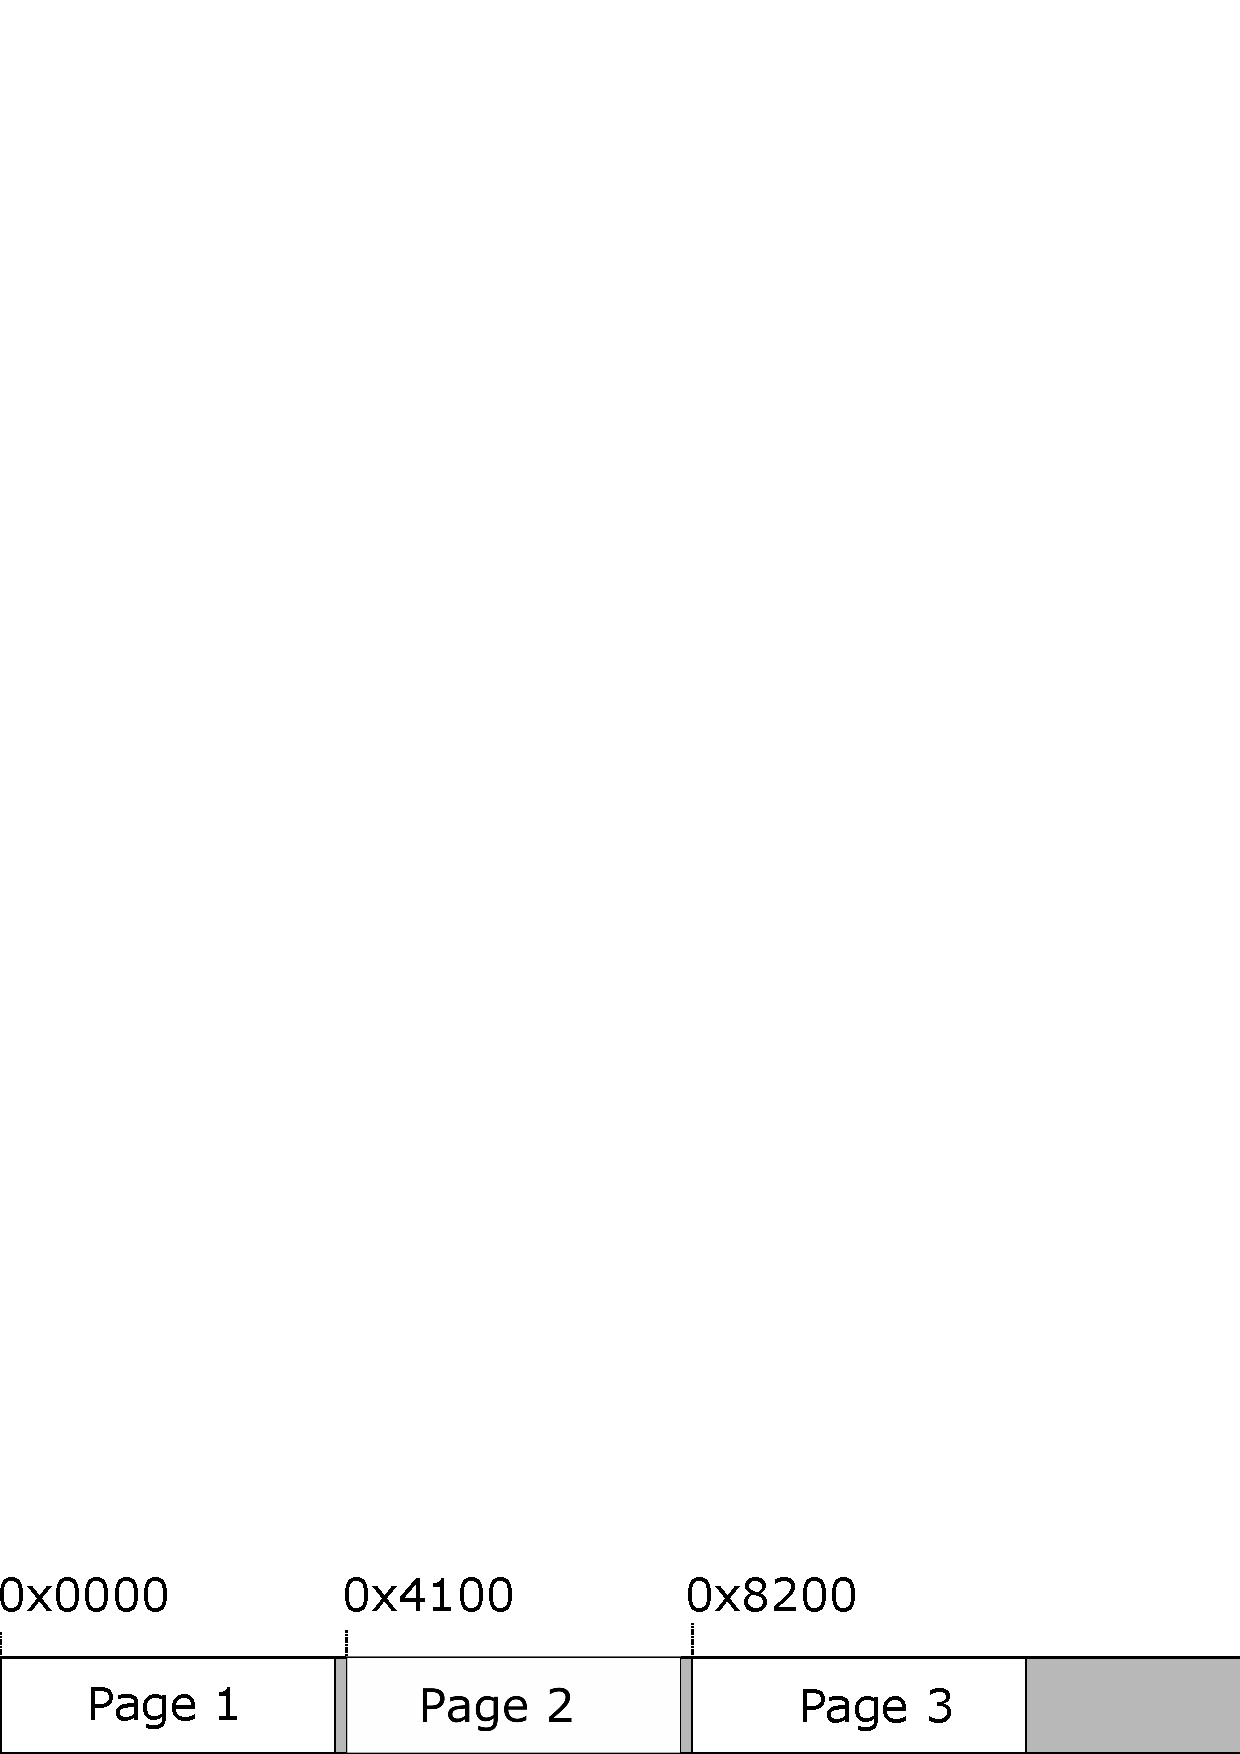
\includegraphics[width=\textwidth]{imgs/drawings/triple_pages_trick_padding.pdf}
\end{figure}
\par



\par
Now page 0 is at 0x0000, page 1 at 0x4100 and page 2 at 0x8200. Moving from any page to an other only requires updating the high 8 bits. Making flipping buffer an atomic operation!\\








\par
\par
DELETE ?\\
Notice how a frame is stored in a page across four banks. Horizontally it looks a little bit like mashed potatoes:
 \begin{figure}[H]
\centering
 \fullimage{vga_layout/intro.png}
 \caption{Intro screen as it appear on screen}
 \end{figure}
 \par
 \begin{figure}[H]
\centering
 \fullimage{vga_layout/intro_bank.png}
 \caption{Intro screen as it is stored across 4 banks in a framebuffer} \label{fig:vga_layout_for_intro}
 \end{figure}
\par
An other example during a 3D sequence.
\begin{figure}[H]
\centering
 \fullimage{vga_layout/wolf3d_7.png}
 \caption{3D View as is appears on screen} \label{fig:vga_layout_in_3D}
 \end{figure}
 \par

 \begin{figure}[H]
\centering
 \fullimage{vga_layout/wolf3d_7_bank.png}
 \caption{3D View as it is stored across 4 banks in a framebuffer}
 \end{figure}
But vertically each bank stores a column intact. This is an important property which is exploited later during the game.
\par













\subsection{Profound Carnage}
After the signon screen comes a second one: the "rating" screen. There were no official rating for video games in 1991 since the ESRB would be established in 1994 in response to criticism of controversial video games with excessively violent (a.k.a Doom) or sexual content. But the team came up with their own self-proclaimed PC-13: The now legendary "Profound Carnage-13".\\
\begin{figure}[H]
\centering
\fullimage{pg13.png}
\end{figure}







\end{document}
